% Options for packages loaded elsewhere
\PassOptionsToPackage{unicode}{hyperref}
\PassOptionsToPackage{hyphens}{url}
%
\documentclass[
]{article}
\usepackage{amsmath,amssymb}
\usepackage{lmodern}
\usepackage{iftex}
\ifPDFTeX
  \usepackage[T1]{fontenc}
  \usepackage[utf8]{inputenc}
  \usepackage{textcomp} % provide euro and other symbols
\else % if luatex or xetex
  \usepackage{unicode-math}
  \defaultfontfeatures{Scale=MatchLowercase}
  \defaultfontfeatures[\rmfamily]{Ligatures=TeX,Scale=1}
\fi
% Use upquote if available, for straight quotes in verbatim environments
\IfFileExists{upquote.sty}{\usepackage{upquote}}{}
\IfFileExists{microtype.sty}{% use microtype if available
  \usepackage[]{microtype}
  \UseMicrotypeSet[protrusion]{basicmath} % disable protrusion for tt fonts
}{}
\makeatletter
\@ifundefined{KOMAClassName}{% if non-KOMA class
  \IfFileExists{parskip.sty}{%
    \usepackage{parskip}
  }{% else
    \setlength{\parindent}{0pt}
    \setlength{\parskip}{6pt plus 2pt minus 1pt}}
}{% if KOMA class
  \KOMAoptions{parskip=half}}
\makeatother
\usepackage{xcolor}
\IfFileExists{xurl.sty}{\usepackage{xurl}}{} % add URL line breaks if available
\IfFileExists{bookmark.sty}{\usepackage{bookmark}}{\usepackage{hyperref}}
\hypersetup{
  pdftitle={BFISH Length Comp Investigations},
  pdfauthor={Meg Oshima},
  hidelinks,
  pdfcreator={LaTeX via pandoc}}
\urlstyle{same} % disable monospaced font for URLs
\usepackage[margin=1in]{geometry}
\usepackage{graphicx}
\makeatletter
\def\maxwidth{\ifdim\Gin@nat@width>\linewidth\linewidth\else\Gin@nat@width\fi}
\def\maxheight{\ifdim\Gin@nat@height>\textheight\textheight\else\Gin@nat@height\fi}
\makeatother
% Scale images if necessary, so that they will not overflow the page
% margins by default, and it is still possible to overwrite the defaults
% using explicit options in \includegraphics[width, height, ...]{}
\setkeys{Gin}{width=\maxwidth,height=\maxheight,keepaspectratio}
% Set default figure placement to htbp
\makeatletter
\def\fps@figure{htbp}
\makeatother
\setlength{\emergencystretch}{3em} % prevent overfull lines
\providecommand{\tightlist}{%
  \setlength{\itemsep}{0pt}\setlength{\parskip}{0pt}}
\setcounter{secnumdepth}{-\maxdimen} % remove section numbering
\usepackage{booktabs}
\usepackage{longtable}
\usepackage{array}
\usepackage{multirow}
\usepackage{wrapfig}
\usepackage{float}
\usepackage{colortbl}
\usepackage{pdflscape}
\usepackage{tabu}
\usepackage{threeparttable}
\usepackage{threeparttablex}
\usepackage[normalem]{ulem}
\usepackage{makecell}
\usepackage{xcolor}
\usepackage{amsmath}
\usepackage{caption}
\ifLuaTeX
  \usepackage{selnolig}  % disable illegal ligatures
\fi

\title{BFISH Length Comp Investigations}
\author{Meg Oshima}
\date{5/21/2021}

\begin{document}
\maketitle

\hypertarget{camera-lengths}{%
\subsection{Camera Lengths}\label{camera-lengths}}

\begin{verbatim}
##        X              PSU          DROP_CD           SPECIES_CD       
##  Min.   :  1.0   Min.   :   18   Length:976         Length:976        
##  1st Qu.:244.8   1st Qu.: 8961   Class :character   Class :character  
##  Median :488.5   Median :23017   Mode  :character   Mode  :character  
##  Mean   :488.5   Mean   :21961                                        
##  3rd Qu.:732.2   3rd Qu.:35943                                        
##  Max.   :976.0   Max.   :45499                                        
##  SCIENTIFIC_NAME    COMMON_NAME           BFISH           OFFICIAL_DEPTH_M
##  Length:976         Length:976         Length:976         Min.   : 77.16  
##  Class :character   Class :character   Class :character   1st Qu.:114.76  
##  Mode  :character   Mode  :character   Mode  :character   Median :152.00  
##                                                           Mean   :155.41  
##                                                           3rd Qu.:192.00  
##                                                           Max.   :274.00  
##    LENGTH_CM         Island         
##  Min.   :  5.40   Length:976        
##  1st Qu.: 25.73   Class :character  
##  Median : 37.34   Mode  :character  
##  Mean   : 38.30                     
##  3rd Qu.: 51.73                     
##  Max.   :111.60
\end{verbatim}

\begin{verbatim}
## Warning: Removed 1 rows containing non-finite values (stat_density).
\end{verbatim}

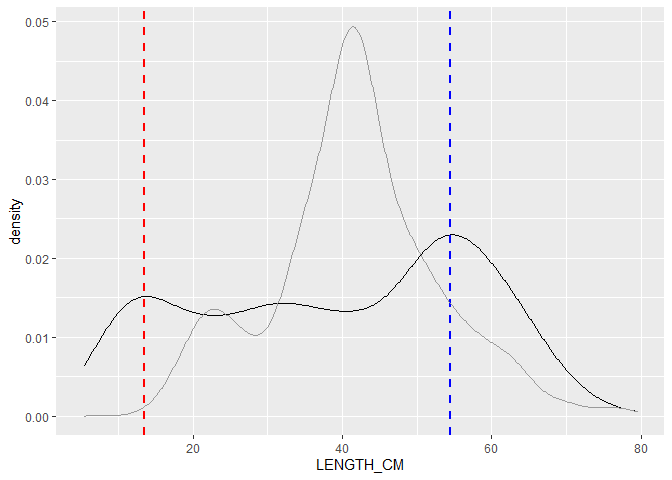
\includegraphics{BFISH_Length_Comp_files/figure-latex/unnamed-chunk-3-1.pdf}

\hypertarget{what-is-causing-the-mode-in-the-smaller-size-classes-in-the-bfish-camera-data}{%
\paragraph{What is causing the mode in the smaller size classes in the
BFISH camera
data?}\label{what-is-causing-the-mode-in-the-smaller-size-classes-in-the-bfish-camera-data}}

\begin{itemize}
\tightlist
\item
  Which sites are most of these samples coming from?
\item
  Which islands are these samples from?\\
\item
  What depth are these samples from?
\end{itemize}

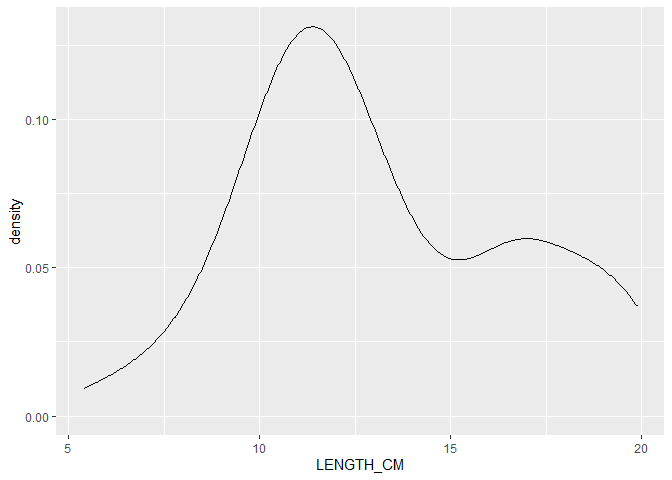
\includegraphics{BFISH_Length_Comp_files/figure-latex/unnamed-chunk-4-1.pdf}
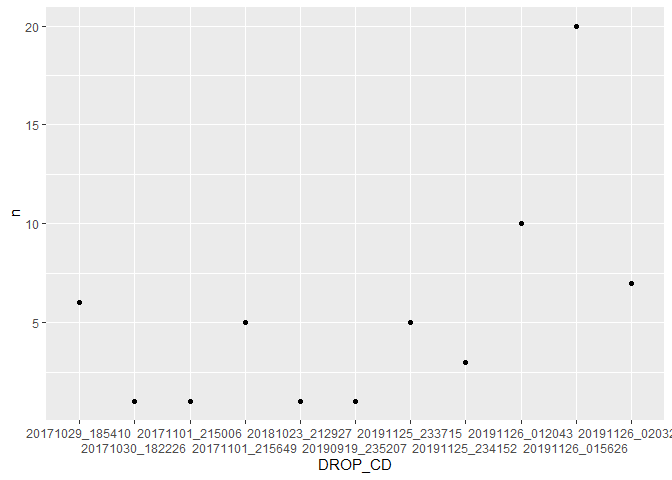
\includegraphics{BFISH_Length_Comp_files/figure-latex/unnamed-chunk-4-2.pdf}

\hypertarget{sites-that-caught-5-or-more-fish-less-than-20cm}{%
\paragraph{Sites that caught 5 or more fish less than
20cm}\label{sites-that-caught-5-or-more-fish-less-than-20cm}}

\captionsetup[table]{labelformat=empty,skip=1pt}
\begin{longtable}{lc}
\toprule
DROP\_CD & n \\ 
\midrule
20191126\_015626 & 20 \\ 
20191126\_012043 & 12 \\ 
20171029\_185410 & 7 \\ 
20191126\_020320 & 7 \\ 
20191125\_233715 & 6 \\ 
20171101\_215649 & 5 \\ 
\bottomrule
\end{longtable}

\begin{figure}
\centering
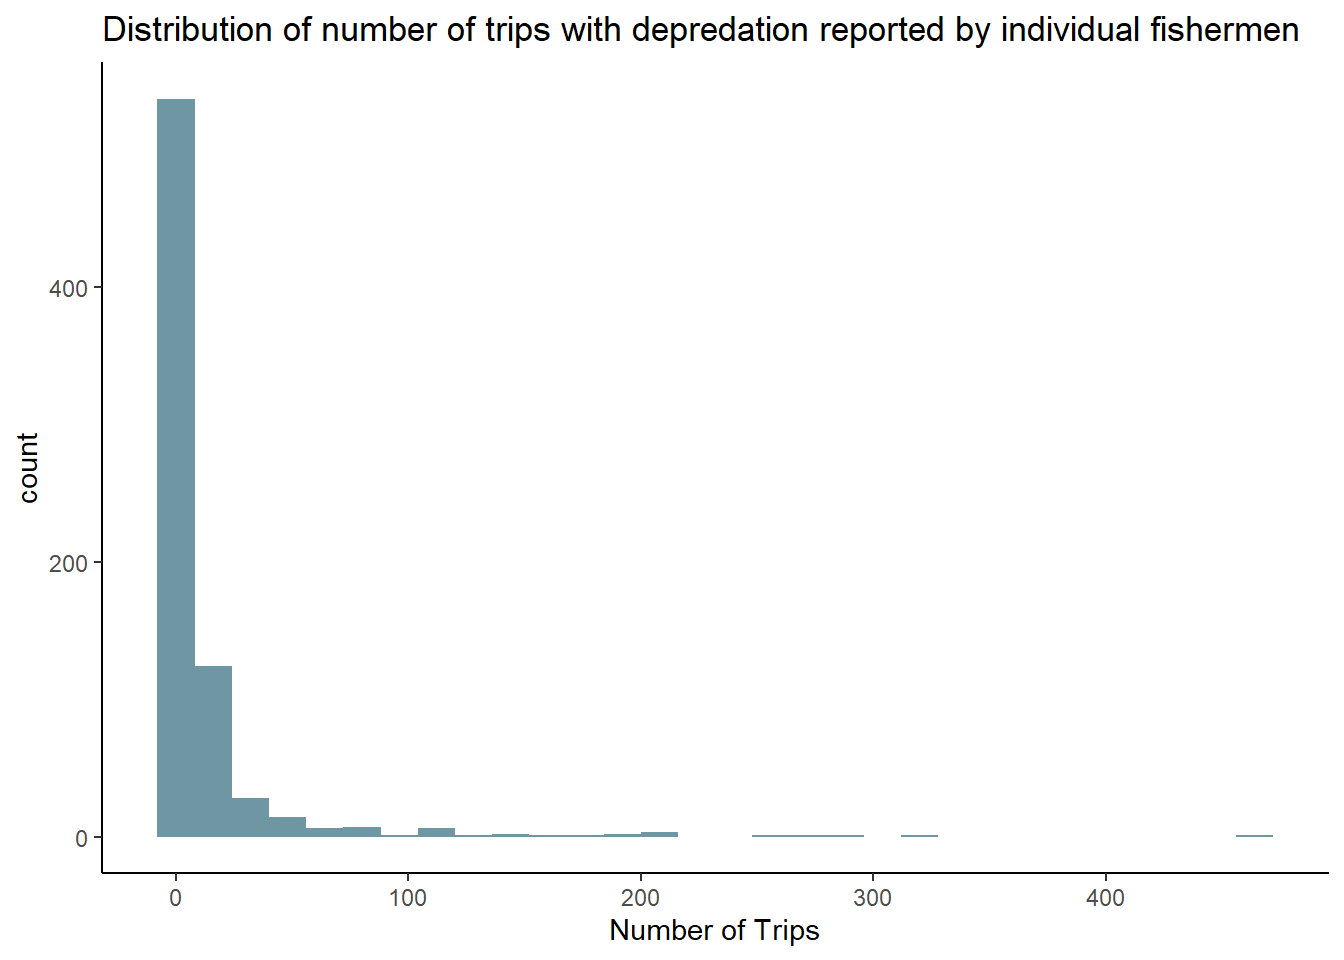
\includegraphics{BFISH_Length_Comp_files/figure-latex/unnamed-chunk-6-1.pdf}
\caption{6 camera drops had 5 or more fish between 10 - 15 cm. The
samples came from Oahu and all were caught between 100 - 110 m deep
(which is the first quantile of depths sampled).}
\end{figure}

\hypertarget{what-is-causing-the-mode-in-the-larger-size-classes-in-the-bfish-camera-data}{%
\paragraph{What is causing the mode in the larger size classes in the
BFISH camera
data?}\label{what-is-causing-the-mode-in-the-larger-size-classes-in-the-bfish-camera-data}}

\begin{itemize}
\tightlist
\item
  Which sites are most of these samples coming from?
\item
  Which islands are these samples from?\\
\item
  What depth are these samples from?
\end{itemize}

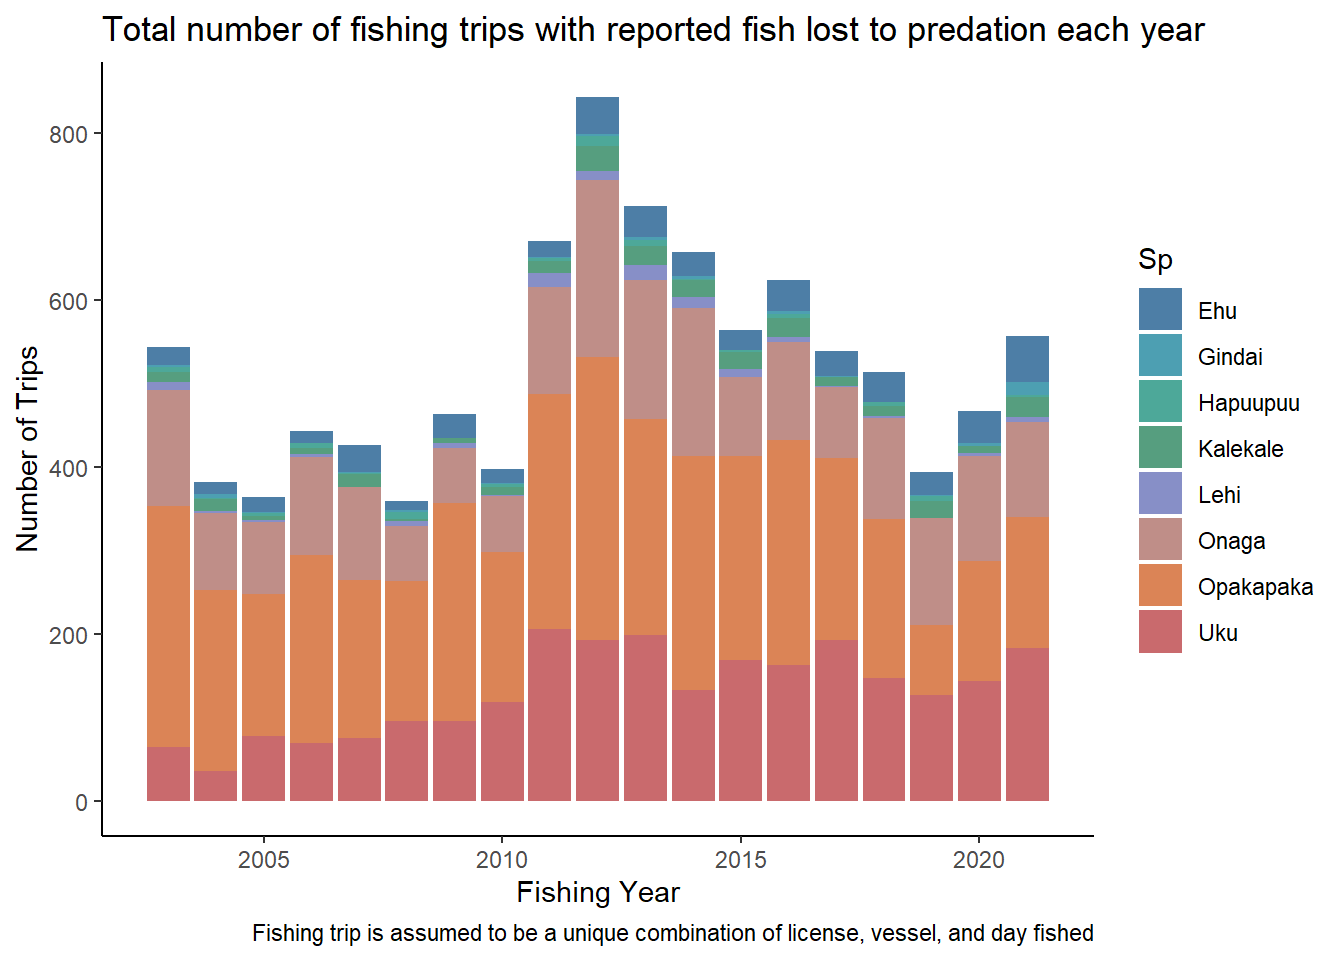
\includegraphics{BFISH_Length_Comp_files/figure-latex/unnamed-chunk-7-1.pdf}
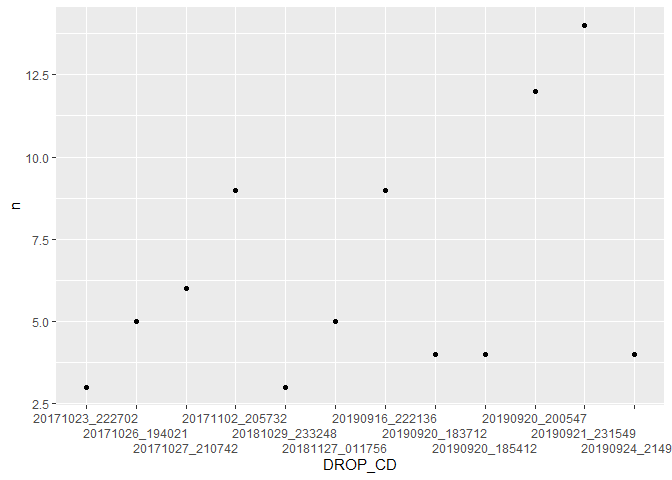
\includegraphics{BFISH_Length_Comp_files/figure-latex/unnamed-chunk-7-2.pdf}

\hypertarget{sites-that-caught-more-than-5-fish-between-50-and-60-cm}{%
\paragraph{Sites that caught more than 5 fish between 50 and 60
cm}\label{sites-that-caught-more-than-5-fish-between-50-and-60-cm}}

\captionsetup[table]{labelformat=empty,skip=1pt}
\begin{longtable}{lc}
\toprule
DROP\_CD & n \\ 
\midrule
20190921\_231549 & 14 \\ 
20190920\_200547 & 12 \\ 
20171102\_205732 & 9 \\ 
20190916\_222136 & 9 \\ 
20171027\_210742 & 6 \\ 
\bottomrule
\end{longtable}

\begin{figure}
\centering
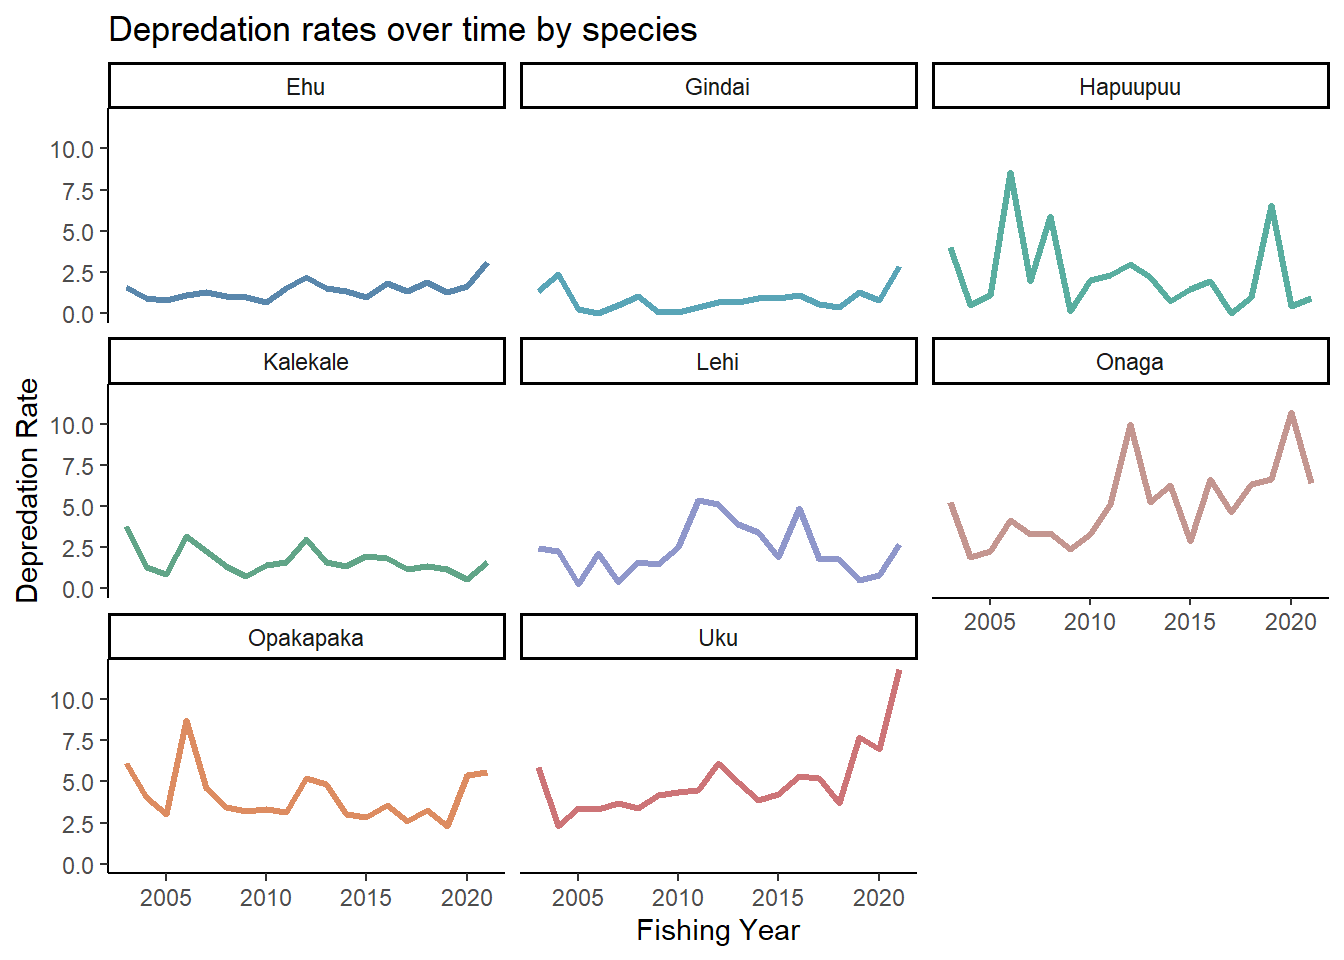
\includegraphics{BFISH_Length_Comp_files/figure-latex/unnamed-chunk-9-1.pdf}
\caption{5 camera drops had more than 5 fish between 50 and 60 cm. The
samples came from the Big Island (n = 1), Kauai (n = 1), Maui Nui (n =
2), and Oahu (n =1) were caught at depths of 150 to 210 m. The two
highest catches occurred in 2019, and all occurred in 2019 or 2017.}
\end{figure}

\hypertarget{fishing-lengths}{%
\subsection{Fishing Lengths}\label{fishing-lengths}}

\begin{verbatim}
##       PSU         SAMPLE_ID          SPECIES_CD        SCIENTIFIC_NAME   
##  Min.   :  271   Length:293         Length:293         Length:293        
##  1st Qu.:11839   Class :character   Class :character   Class :character  
##  Median :16916   Mode  :character   Mode  :character   Mode  :character  
##  Mean   :19741                                                           
##  3rd Qu.:32422                                                           
##  Max.   :43397                                                           
##                                                                          
##  COMMON_NAME          LENGTH_CM       WEIGHT_LB        BFISH          
##  Length:293         Min.   :16.00   Min.   :0.000   Length:293        
##  Class :character   1st Qu.:35.50   1st Qu.:1.408   Class :character  
##  Mode  :character   Median :41.50   Median :2.546   Mode  :character  
##                     Mean   :41.54   Mean   :3.300                     
##                     3rd Qu.:48.00   3rd Qu.:4.877                     
##                     Max.   :77.00   Max.   :9.900                     
##                     NA's   :1       NA's   :253                       
##  SAMPLE_MEAN_DEPTH_M    Island         
##  Min.   : 79.0       Length:293        
##  1st Qu.:116.0       Class :character  
##  Median :137.0       Mode  :character  
##  Mean   :139.3                         
##  3rd Qu.:158.0                         
##  Max.   :260.0                         
## 
\end{verbatim}

\hypertarget{sites-that-caught-more-than-1-fish-between-20-and-25-cm}{%
\paragraph{Sites that caught more than 1 fish between 20 and 25
cm}\label{sites-that-caught-more-than-1-fish-between-20-and-25-cm}}

\captionsetup[table]{labelformat=empty,skip=1pt}
\begin{longtable}{lc}
\toprule
SAMPLE\_ID & n \\ 
\midrule
201708310930LANA & 5 \\ 
201708310749LANA & 4 \\ 
201910060752JOMO & 4 \\ 
201709101027ROMO & 3 \\ 
\bottomrule
\end{longtable}

\begin{figure}
\centering
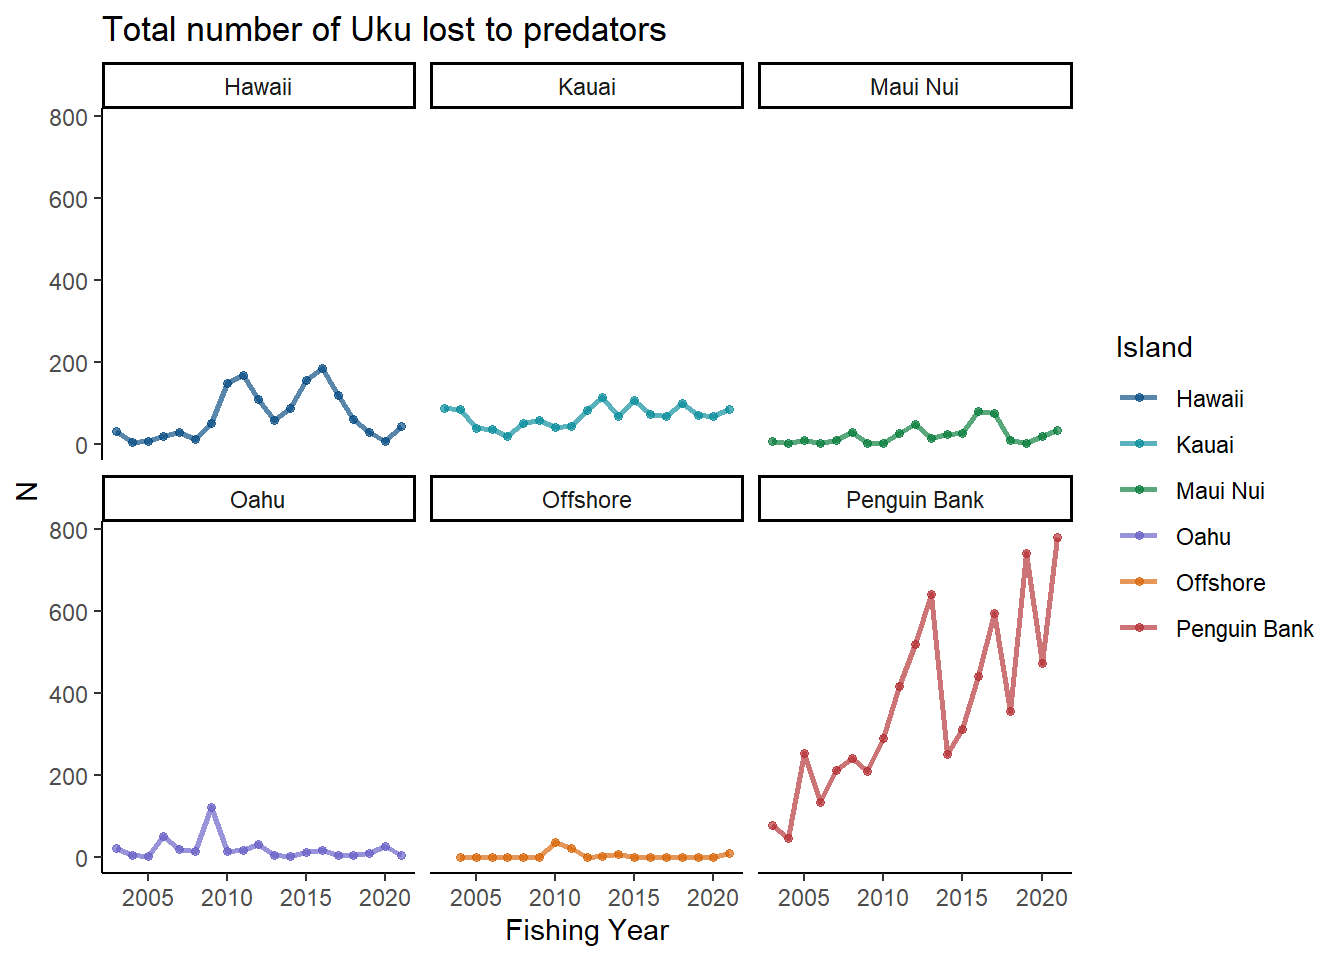
\includegraphics{BFISH_Length_Comp_files/figure-latex/unnamed-chunk-13-1.pdf}
\caption{4 fishing events had more than 1 fish between 20 and 25 cm. The
samples came from Oahu (n = 2) and Maui Nui (n = 2) and were caught at
depths 89 to 142 m. The catches occurred in 2017 (n = 3) and 2019 (n =
1).}
\end{figure}

\hypertarget{camera-lengths-by-island-and-year}{%
\subsection{Camera Lengths by Island and
Year}\label{camera-lengths-by-island-and-year}}

\begin{itemize}
\tightlist
\item
  5 Islands - Big Island, Maui Nui, Oahu, Ni'ihau, Kauai
\item
  4 Years - 2016, 2017, 2018, 2019
\end{itemize}

\hypertarget{number-of-samples-per-year}{%
\paragraph{Number of Samples per
Year}\label{number-of-samples-per-year}}

\captionsetup[table]{labelformat=empty,skip=1pt}
\begin{longtable}{lc}
\toprule
Year & n \\ 
\midrule
2016 & 39 \\ 
2017 & 138 \\ 
2018 & 96 \\ 
2019 & 262 \\ 
\bottomrule
\end{longtable}

\hypertarget{density-plot-by-year}{%
\paragraph{Density Plot by Year}\label{density-plot-by-year}}

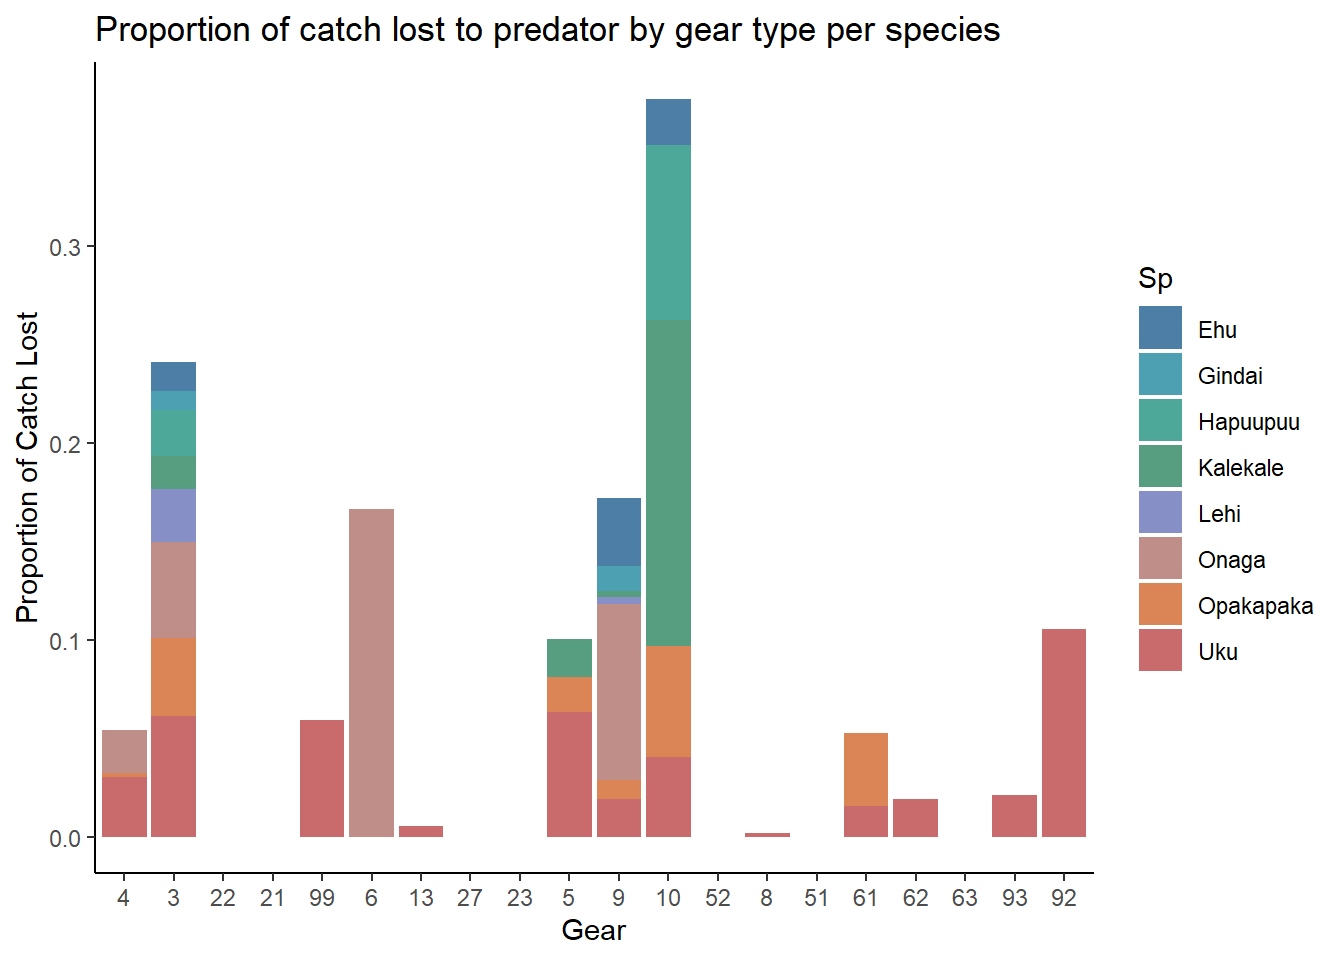
\includegraphics{BFISH_Length_Comp_files/figure-latex/unnamed-chunk-15-1.pdf}

\begin{itemize}
\tightlist
\item
  All years have a bimodal (or tri) distribution, but small modes
  differ.\\
\item
  2019 has three modes, with middle one being the smallest.\\
\item
  2017 and 2018 are very similar to each other and 2016 is the most
  distinct from the other years.
\end{itemize}

\hypertarget{number-of-samples-per-island}{%
\paragraph{Number of Samples per
Island}\label{number-of-samples-per-island}}

\captionsetup[table]{labelformat=empty,skip=1pt}
\begin{longtable}{cc}
\toprule
Island & n \\ 
\midrule
Maui Nui & 209 \\ 
Big Island & 157 \\ 
Oahu & 120 \\ 
Kauai & 39 \\ 
Niihau & 10 \\ 
\bottomrule
\end{longtable}

\hypertarget{density-plot-by-island}{%
\paragraph{Density Plot by Island}\label{density-plot-by-island}}

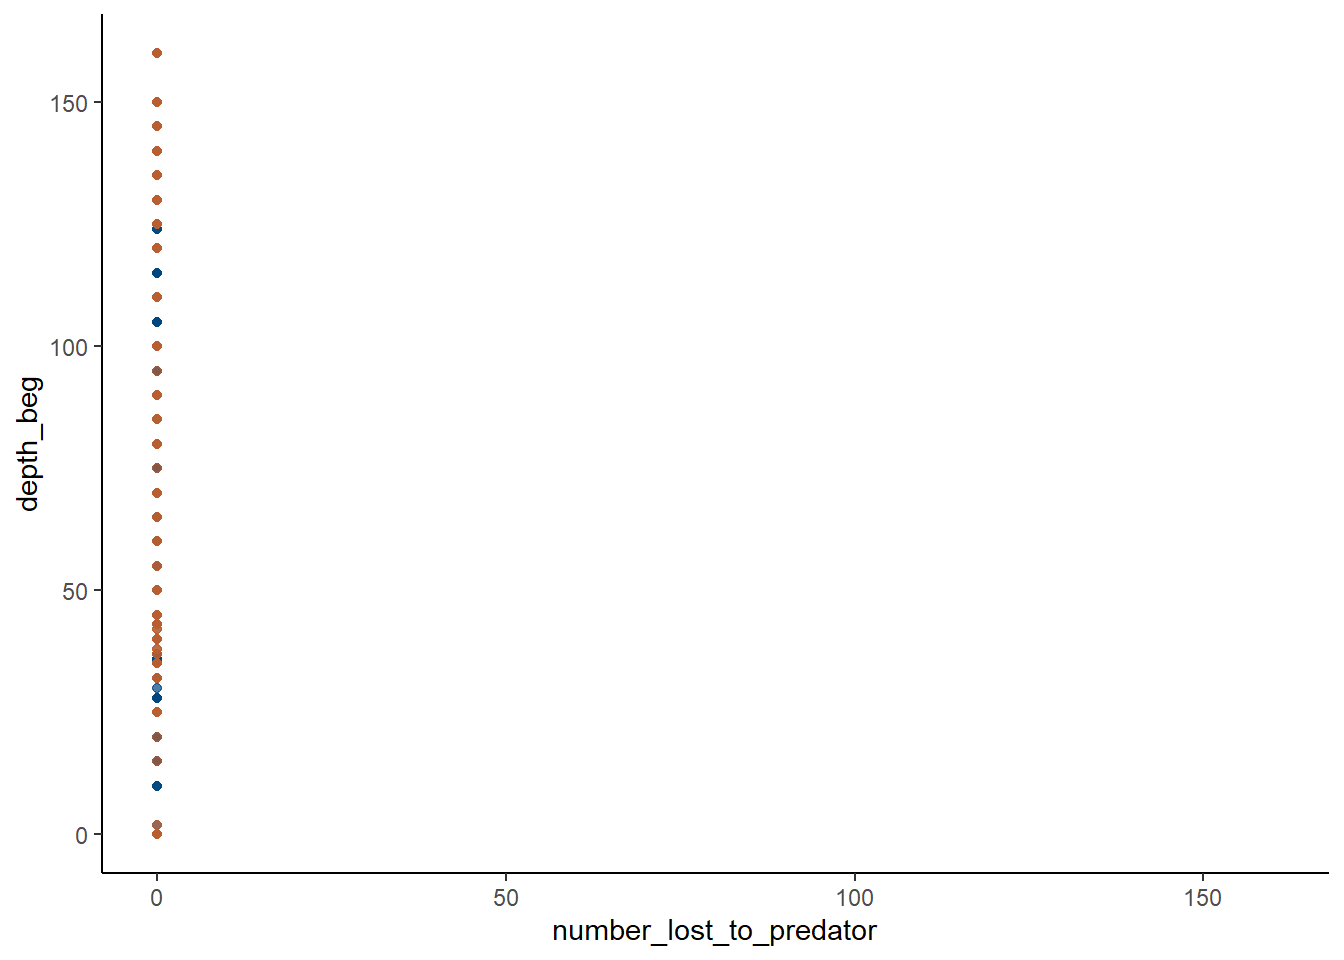
\includegraphics{BFISH_Length_Comp_files/figure-latex/unnamed-chunk-17-1.pdf}

\begin{itemize}
\tightlist
\item
  Big Island and Oahu have more smaller fish and less bigger fish than
  the other islands.\\
\item
  Niihau only had larger fish.\\
\item
  Kauai had an almost even split between smaller and larger fish (with
  bigger small fish so less of a difference between modes).
\end{itemize}

\hypertarget{number-of-samples-per-islandyear}{%
\paragraph{Number of Samples per
Island/Year}\label{number-of-samples-per-islandyear}}

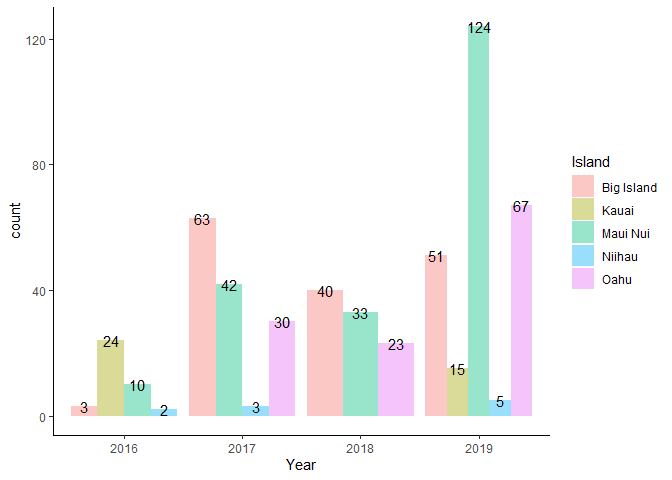
\includegraphics{BFISH_Length_Comp_files/figure-latex/unnamed-chunk-18-1.pdf}

\hypertarget{density-plot-by-island-and-year}{%
\paragraph{Density Plot by Island and
Year}\label{density-plot-by-island-and-year}}

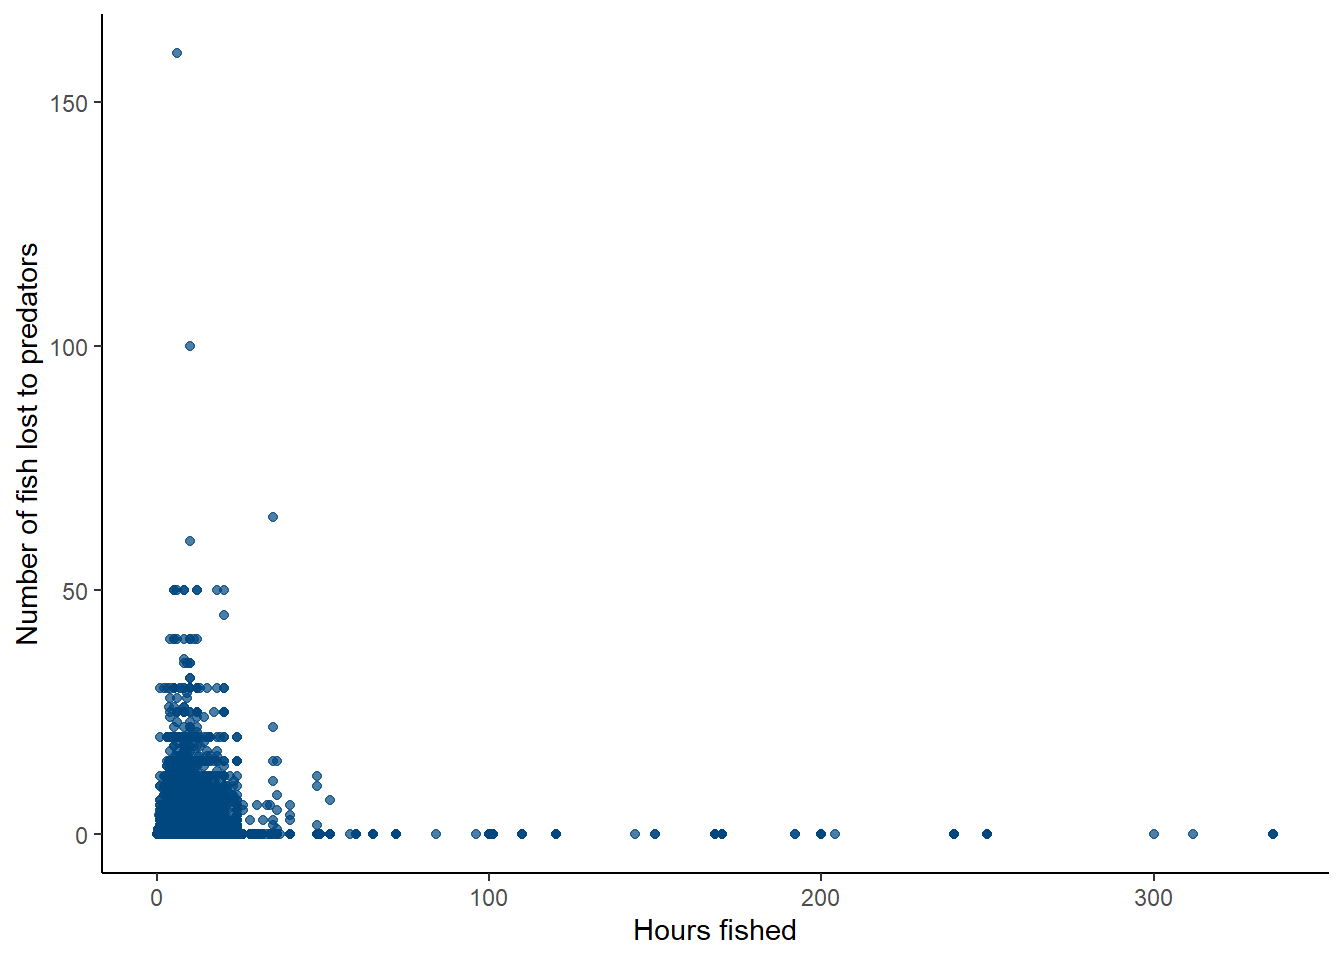
\includegraphics{BFISH_Length_Comp_files/figure-latex/unnamed-chunk-19-1.pdf}

\begin{itemize}
\tightlist
\item
  In the Big Island, catches were pretty consistent between 2017-2019
  but 2016 was very different, probably because n = 3. Also, depth was
  more in the mid-range of sampled depths. They did not sample in the
  shallower range, unlike other years.\\
\item
  Kauai only had 2 years of data (2016 n = 24, and 2019 n = 15) and the
  distributions were different, 2016 had mostly smaller fish whereas
  2019 had more larger fish.\\
\item
  Maui Nui catches all had the same mode for larger sizes (between 40 -
  70 cm) but the modes for the smaller sized fish fluctuated each
  year.\\
\item
  Niihau had very small sample sizes (n = 2 - 5) for the 3 years
  sampling occurred there so distributions are not that reliable but
  size range is fairly consistent. Also, the distributions are
  consistent with the 2019 lengths in Kauai (support for combining those
  regions?).\\
\item
  Oahu had consistent length distributions for 2017 and 2018 but 2019
  was almost exclusively small fish (\textless{} 20 cm, n = 67)
\end{itemize}

\hypertarget{density-plot-by-year-and-island}{%
\paragraph{Density Plot by Year and
Island}\label{density-plot-by-year-and-island}}

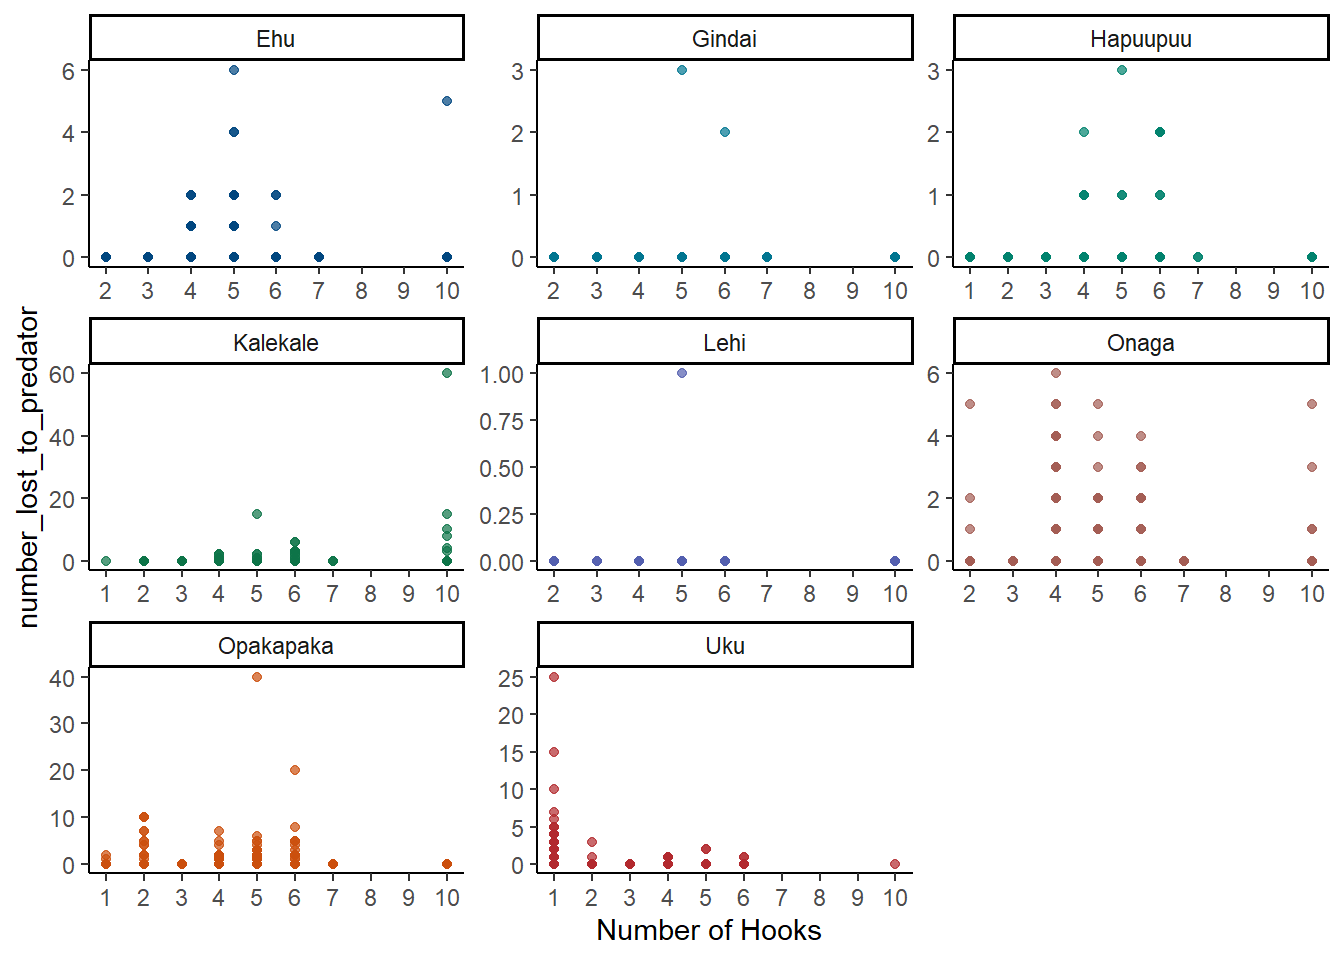
\includegraphics{BFISH_Length_Comp_files/figure-latex/unnamed-chunk-20-1.pdf}

\begin{itemize}
\tightlist
\item
  In 2016, Big Island (n = 3) and Kauai (n = 24) were similar and Niiahu
  (n = 2) and Maui Nui (n = 10) were similar.\\
\item
  In 2017, mostly smaller fish caught off Big Island compared to the
  other islands.
\item
  In 2018, there is a bimodal distribution for Maui Nui and less
  pronouced for the Big Island. Oahu has only larger fish
  (\textgreater{} 40 cm).\\
\item
  In 2019, the first mode is almost exclusively from Oahu samples, the
  second mode is from Big Island and Maui Nui samples, and the third
  mode is from all islands.
\end{itemize}

\captionsetup[table]{labelformat=empty,skip=1pt}
\begin{longtable}{lrrrrr}
\caption*{
\large Sampled Depths\\ 
\small \\ 
} \\ 
\toprule
 & min & Q1 & Q2 & Q3 & max \\ 
\midrule
\multicolumn{1}{l}{Big Island} \\ 
\midrule
2016 & $123.91$ & $152.16$ & $180.41$ & $189.41$ & $198.41$ \\ 
2017 & $82.00$ & $110.00$ & $130.00$ & $138.50$ & $203.00$ \\ 
2018 & $97.00$ & $121.25$ & $134.00$ & $154.00$ & $224.00$ \\ 
2019 & $91.88$ & $94.38$ & $94.56$ & $143.48$ & $223.89$ \\ 
\midrule
\multicolumn{1}{l}{Kauai} \\ 
\midrule
2016 & $114.03$ & $114.03$ & $114.03$ & $114.03$ & $177.28$ \\ 
2019 & $160.56$ & $160.56$ & $160.56$ & $160.56$ & $160.56$ \\ 
\midrule
\multicolumn{1}{l}{Maui Nui} \\ 
\midrule
2016 & $91.41$ & $138.22$ & $166.56$ & $185.27$ & $203.56$ \\ 
2017 & $95.00$ & $108.00$ & $131.00$ & $194.00$ & $238.00$ \\ 
2018 & $102.00$ & $111.00$ & $111.00$ & $141.00$ & $180.00$ \\ 
2019 & $102.94$ & $112.06$ & $146.29$ & $154.56$ & $202.16$ \\ 
\midrule
\multicolumn{1}{l}{Niihau} \\ 
\midrule
2016 & $149.78$ & $149.78$ & $149.78$ & $149.78$ & $149.78$ \\ 
2017 & $148.00$ & $148.00$ & $148.00$ & $191.50$ & $235.00$ \\ 
2019 & $111.69$ & $111.69$ & $111.69$ & $113.03$ & $113.03$ \\ 
\midrule
\multicolumn{1}{l}{Oahu} \\ 
\midrule
2017 & $139.00$ & $177.00$ & $210.00$ & $210.00$ & $210.00$ \\ 
2018 & $95.00$ & $126.00$ & $133.00$ & $192.00$ & $210.00$ \\ 
2019 & $79.81$ & $79.81$ & $101.19$ & $107.44$ & $126.81$ \\ 
\bottomrule
\end{longtable}

\end{document}
